\documentclass[10pt,a4paper]{article}
\usepackage[utf8]{inputenc}
\usepackage[frenchb]{babel}
\usepackage[T1]{fontenc}
\usepackage{graphicx}
\usepackage{fancyhdr}
\usepackage{eurosym}

\lhead{Manuel d'utilisation de votre site Internet}
\rhead {Rémy Mondi (iMaugis)}
\lfoot{
\includegraphics[scale=0.5]{img/cc-by-nc-sa.png}}
\cfoot{}
\rfoot{Page \thepage}

\pagestyle{fancy}

\title{Manuel d'utilisation de votre site Internet}
\author{Rémy Mondi (iMaugis)}
\date{\today}

\begin{document}

\maketitle
\begin{figure}[!h]
\begin{center}

\includegraphics[scale=0.5]{img/logo-imaugis.png}
\end{center}
\end{figure}
\newpage

\tableofcontents
\newpage

\part{Premiers pas avec votre site}
\newpage

\section{Tour d'horizon de votre site}
\paragraph{}Votre site se décompose en deux partie principales : le front-office et le back-office.
\subsection{Le "Front-Office"}
\paragraph{}Le front-office est la partie site, la boutique, ce que voient les visiteurs qui viennent sur votre site.
\begin{center}
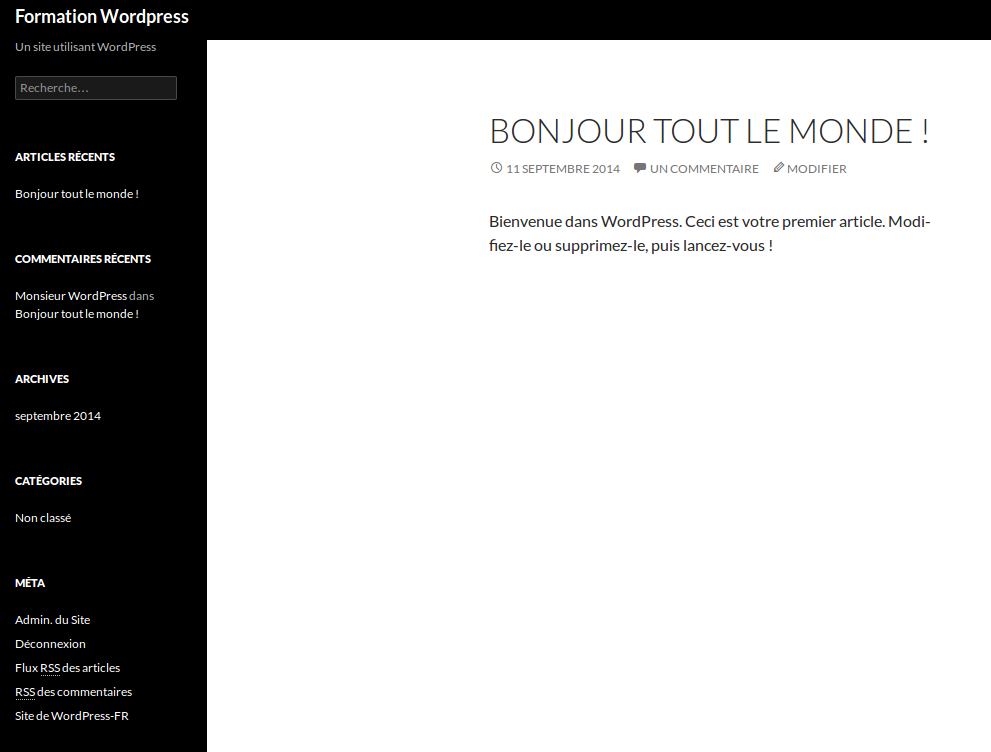
\includegraphics[scale=0.35]{img/0047.png}
\end{center}
\paragraph{}Le front-office affichera ce que vous aurez envie d'afficher c'est vous qui décidez !
\paragraph{}Par exemple : Vos articles, vos menus, vos galeries photos, vos vidéos, un forum de discussion, des sondages, etc...
\paragraph{}Pour accéder au front-office, il suffit d'entrer l'adresse de votre site (celle que vous aura communiquer votre hébergeur) dans la barre d'adresse de votre navigateur.
\paragraph{}Par exemple : http://www.monsite.com

\subsection{Le "Back-Office"}
\paragraph{}Le back-office est la partie administration. C'est l’arrière-boutique de votre site ; l'interface d’administration va permettre de créer et mettre à jour vos articles mais aussi de gérer tout votre site.
\begin{center}
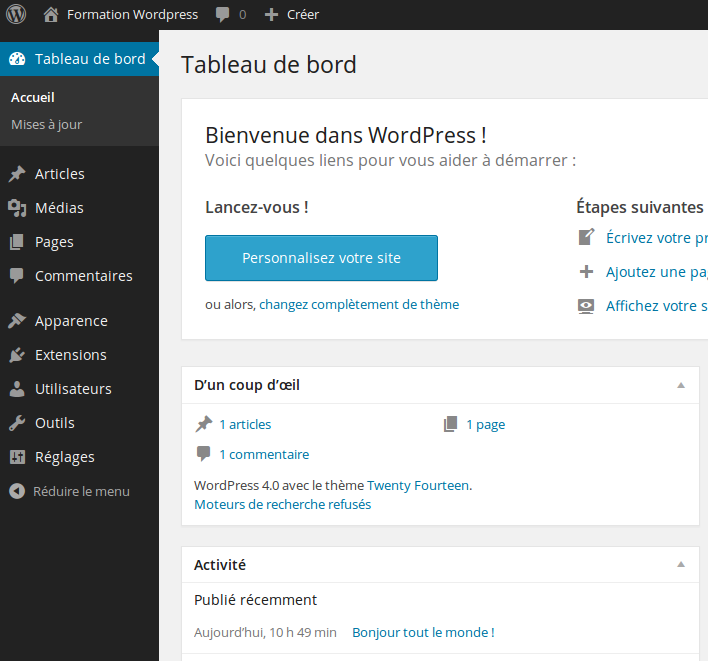
\includegraphics[scale=0.5]{img/0046.png}
\end{center}
\paragraph{}Comme expliqué plus haut, le back-office vous permettra de gérer le site :
\begin{itemize}
\item Ajouter, modifier, supprimer des articles
\item Créer des catégories pour organiser vos articles
\item Ajouter du contenu multimédia (images, sons)
\item Ajouter, modifier, supprimer des menus
\item Gérer les utilisateurs
\item De mettre à jour votre site
\end{itemize}
\paragraph{}Pour accéder au back-office, il suffit d'entrer l'adresse de votre site suivi de « /wp-admin »
\paragraph{}Par exemple : http://www.monsite.com/wp-admin
\newpage

\section{Effectuer les mises à jour de votre site}
\paragraph{}Effectuer les mises à jours que propose votre site et très important. En effet, les mises à jours peuvent corriger des bugs ou des failles de sécurité. Mais vous allez voir que faire ses mises à jour sous votre site est un jeu d'enfant.
\paragraph{}Avant toute chose vous allez déjà vous rendre compte que votre site vous avertit de la présence de mises à jour disponibles. En effet, lorsque vous vous connectez au back-office vous pourrez constater la présence de mises à jour en dessous de l'onglet « Tableau de bord » comme dans les exemples ci-dessous :
\begin{center}
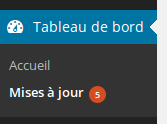
\includegraphics[scale=0.5]{img/0050.png}
\end{center}
\begin{center}
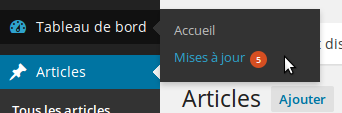
\includegraphics[scale=0.5]{img/0051.png}
\end{center}
\paragraph{}Nous voyons très clairement dans cet exemple que 5 mises à jours sont disponibles.
\paragraph{}Par contre, une chose importante à savoir et qu'il existe 4 types de mises à jour :
\begin{itemize}
\item Les mises à jours du core (cœur) de votre site
\item Les mises à jours des extensions
\item Les mises à jour des thèmes
\item Les mises à jour des traductions
\end{itemize}
\paragraph{}Maintenant que vous savez tout, il n'y a plus qu'à effectuer les mises à jours (s'il y en a à faire bien évidemment…). Pour cela, rien de plus simple, cliquez sur le menu… « Mises à jour ».
\subsection{Mises à jour du core (cœur) de votre site}
\paragraph{}Dans le page des Mises à jour de votre site, en dessous du titre « Une nouvelle version de votre site est disponible » Cliquez sur le bouton « Mettre à jour ».
\begin{center}
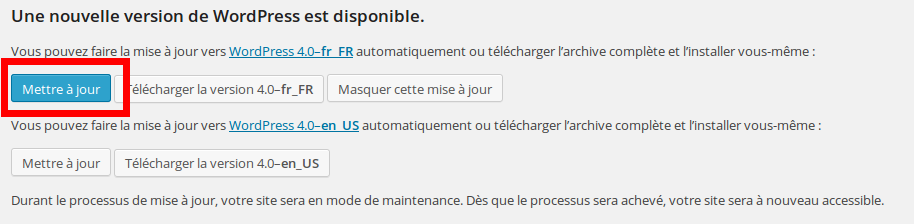
\includegraphics[scale=0.35]{img/0052.png}
\end{center}
\paragraph{}Dans certains, cas une mise à jour peut vous demander de vous reconnecter.
\subsection{Mises à jour des extensions}
\paragraph{}Dans le page des Mises à jour de votre site (lorsque des mises à jour pour les extensions sont disponibles), cliquez sur « Tout sélectionner » en dessous du titre « Extensions » puis cliquez sur le bouton « Mettre à jour les extensions ».
\begin{center}
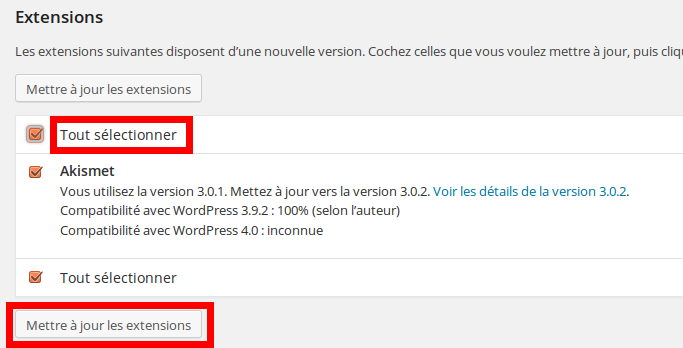
\includegraphics[scale=0.35]{img/0053.png}
\end{center}
\paragraph{}Une fois la mise à jour des extensions terminées cliquez sur le lien « Retourner aux mises à jour de votre site ».
\begin{center}
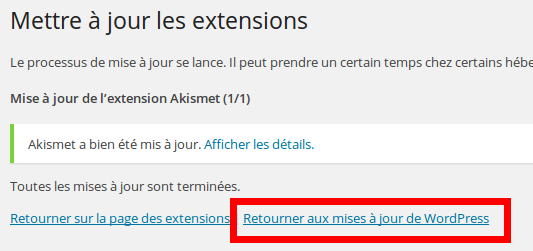
\includegraphics[scale=0.35]{img/0054.png}
\end{center}
\subsection{Mises à jour des thèmes}
\paragraph{}Dans le page des Mises à jour de votre site (lorsque des mises à jour pour les thèmes sont disponibles), cliquez sur « Tout sélectionner » en dessous du titre « Thèmes » puis cliquez sur le bouton « Mettre à jour les thèmes ».
\begin{center}
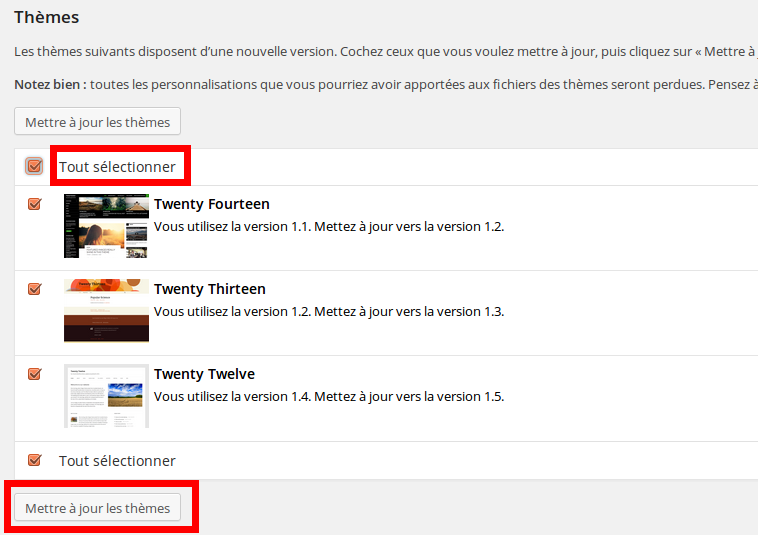
\includegraphics[scale=0.35]{img/0055.png}
\end{center}
\paragraph{}Une fois la mise à jour des thèmes terminées cliquez sur le lien « Retourner aux mises à jour de votre site ».
\begin{center}
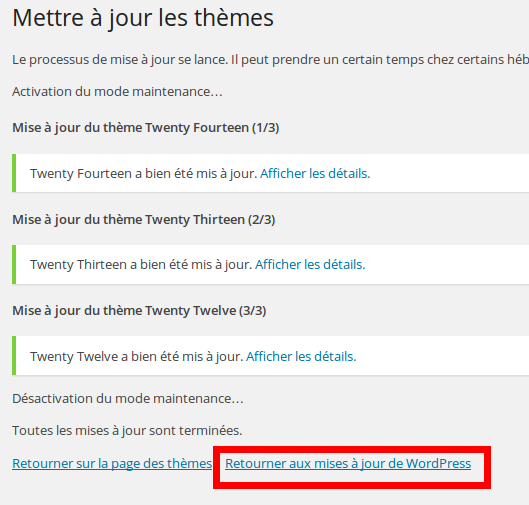
\includegraphics[scale=0.35]{img/0056.png}
\end{center}
\subsection{Mises à jour des traductions}
\paragraph{}Dans le page des Mises à jour de votre site (lorsque des mises à jour pour les traductions sont disponibles), cliquez sur le bouton « Mise à jour des traductions ».
\begin{center}
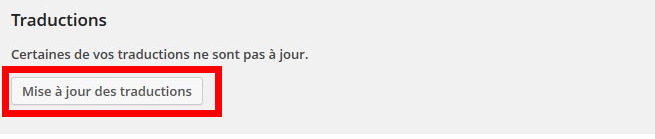
\includegraphics[scale=0.35]{img/0057.png}
\end{center}
\paragraph{}Une fois la mise à jour des traductions terminées cliquez sur le lien « Retourner aux mises à jour de votre site ».
\begin{center}
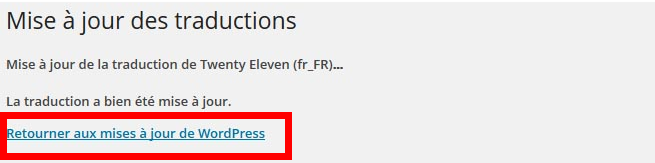
\includegraphics[scale=0.35]{img/0058.png}
\end{center}
\paragraph{}Et voilà, vous avez installé, configuré, et mis a jour votre site ! Maintenant vous pouvez :
\begin{itemize}
\item Ajouter vos contenus
\item et pleins de choses encore !
\end{itemize}
\newpage

\part{Les publications}
\newpage

\section{Les articles et les pages}
\paragraph{} Les contenus sont organisés en deux types : les articles et les pages. La différence entre les deux réside dans le type de contenu que vous allez placer à l’intérieur.
\begin{itemize}
\item \textbf{Un article} sera généralement un contenu d’actualité, c’est-à-dire qu’il prend sa plus grande valeur au moment de sa publication. C’est typiquement le type de contenu utilisé pour les publications d’un blog ou sur un fil d’actualité.
\item \textbf{Une page} aura au contraire un contenu à valeur constante dans le temps sans avoir besoin d’être mise à jour. On peut l’utiliser pour présenter une société, une personne ou bien pour parler d’un sujet de fond.
\end{itemize}
\paragraph{}Au niveau de la présentation, les articles peuvent être affichés en liste par ordre chronologique, puisque c’est ce qui fait leur sens, soit complètement soit avec un aperçu du contenu, tandis que les pages seront accessibles par un lien (le plus souvent dans le menu de navigation) vers leur contenu.
\subsection{Lister les articles et les pages}
\paragraph{}Pour lister les articles, cliquez sur le bouton « Articles » dans le menu de gauche de votre site.
\begin{center}

\includegraphics[scale=0.5]{img/0059.png}
\end{center}
\paragraph{}Vous obtiendrez alors la liste complète des articles présents sur votre site. Ces articles sont triés par défaut du plus récent au plus ancien.
\begin{center}
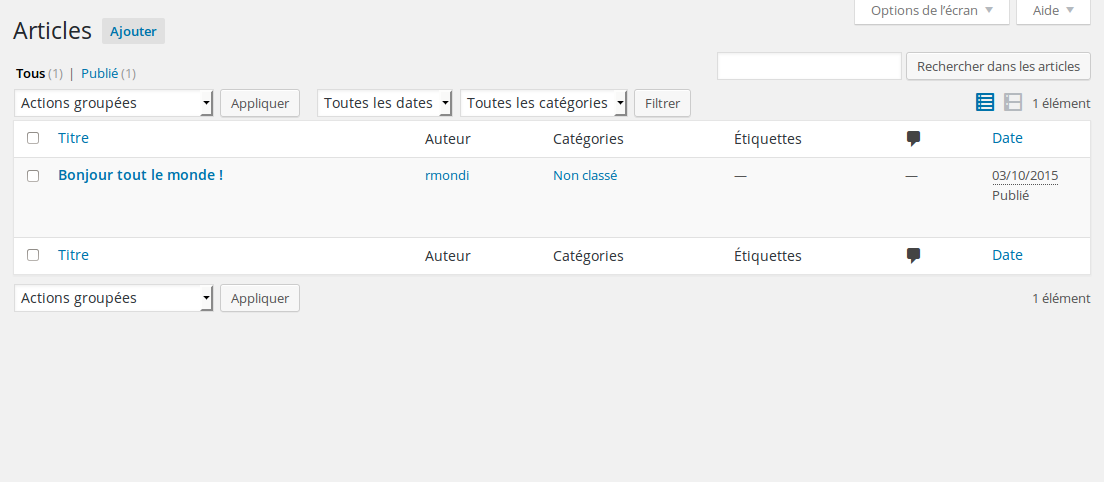
\includegraphics[scale=0.3]{img/0060.png}
\end{center}
\paragraph{}Pour lister les pages, cliquez sur le bouton « Pages » dans le menu de gauche de votre site.
\begin{center}

\includegraphics[scale=0.5]{img/0061.png}
\end{center}
\paragraph{}Vous obtiendrez alors la liste complète des pages présentes sur votre site. Ces pages sont triées par défaut de la plus récente à la plus ancienne.
\begin{center}
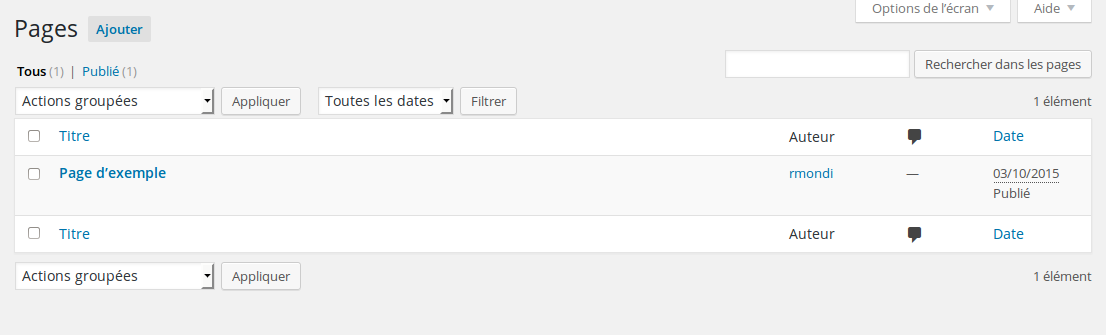
\includegraphics[scale=0.3]{img/0062.png}
\end{center}
\subsection{Ajouter, éditer ou supprimer un article ou une page}
\subsubsection{Ajouter un article ou une page}
\paragraph{}Pour ajouter un nouvel article ou une nouvelle page, cliquez sur... « Ajouter ».
\begin{center}
\begin{tabular}{cc}

\includegraphics[scale=0.35]{img/0063.png} &
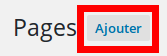
\includegraphics[scale=0.4]{img/0065.png} \\
\end{tabular}
\end{center}
\paragraph{}Vous obtiendrez un formulaire pour écrire un nouvel article ou une nouvelle page.
\begin{center}
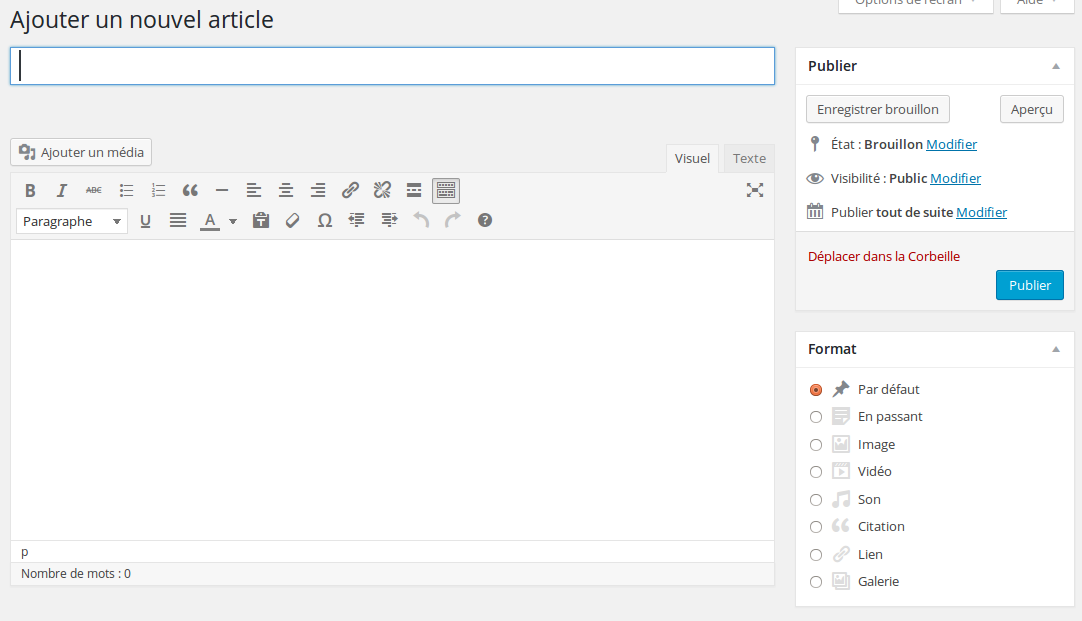
\includegraphics[scale=0.3]{img/0064.png}
\end{center}
\subsubsection{Éditer un article ou une page}
\paragraph{}Pour éditer un article ou une page, passez votre souris sur l'article ou la page en question afin de faire apparaître des options supplémentaires. Cliquez ensuite sur « Modifier ».
\begin{center}
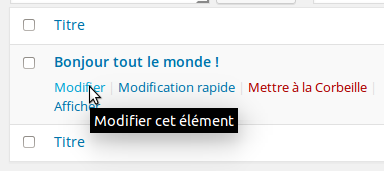
\includegraphics[scale=0.35]{img/0066.png}
\end{center}
\paragraph{}Vous obtiendrez le formulaire pour éditer votre article ou votre page.
\begin{center}
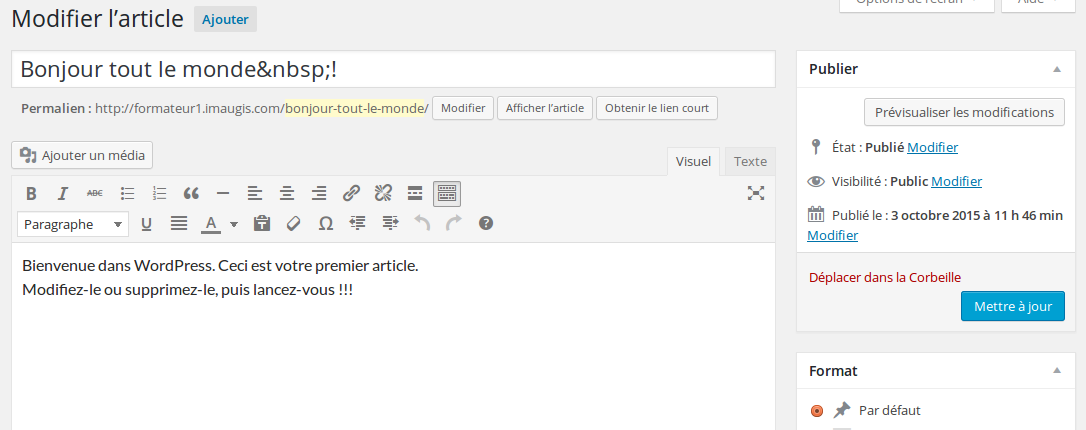
\includegraphics[scale=0.35]{img/0067.png}
\end{center}
\subsubsection{Supprimer un article ou une page}
\paragraph{}Pour supprimer un article ou une page, passez votre souris sur l'article ou la page en question afin de faire apparaître des options supplémentaires. Cliquez ensuite sur « Mettre à la corbeille ».
\begin{center}
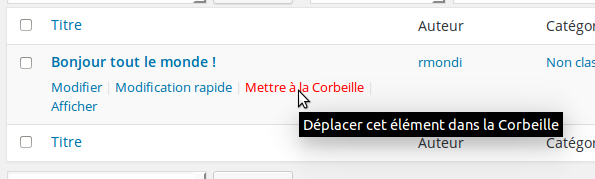
\includegraphics[scale=0.35]{img/0068.png}
\end{center}
\paragraph{}Il est important de préciser que l'action « Mettre à la corbeille » n'est pas irréversible. En effet, vous pouvez rétablir un article ou une page, que vous auriez supprimé accidentellement par exemple, dans la corbeille.
\paragraph{}Si votre corbeille contient au moins un élément, vous verrez alors apparaître « Corbeille » suivi du nombre d'éléments qu'elle contient entre parenthèses au-dessus de la liste de vos articles ou pages.
\paragraph{}Cliquez sur le bouton « Corbeille » pour afficher la liste des articles ou pages qu'elle contient.
\begin{center}
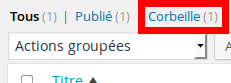
\includegraphics[scale=0.35]{img/0069.png}
\end{center}
\paragraph{}Passez votre souris sur un article ou une page pour faire apparaître des options supplémentaires et cliquez sur « Rétablir » si vous souhaitez... rétablir un article ou une page supprimés accidentellement ou bien cliquez sur « Supprimer définitivement » si vous souhaitez... supprimer définitivement un article ou une page.
\paragraph{}À noter que vous pouvez \textbf{supprimer définitivement} le contenu de la corbeille en cliquant sur le bouton « Vider la corbeille ».
\begin{center}
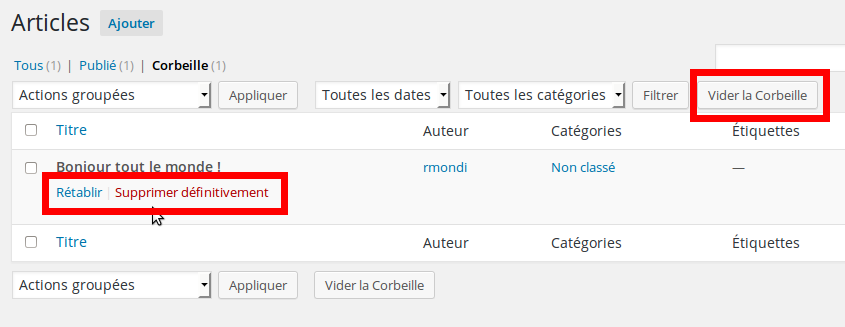
\includegraphics[scale=0.35]{img/0070.png}
\end{center}
\subsection{Le formatage d'un article ou d'une page}
\subsubsection{Les paragraphes}
\paragraph{} Le paragraphe est le formatage de texte par défaut dans l'éditeur de texte de votre site.
\begin{center}
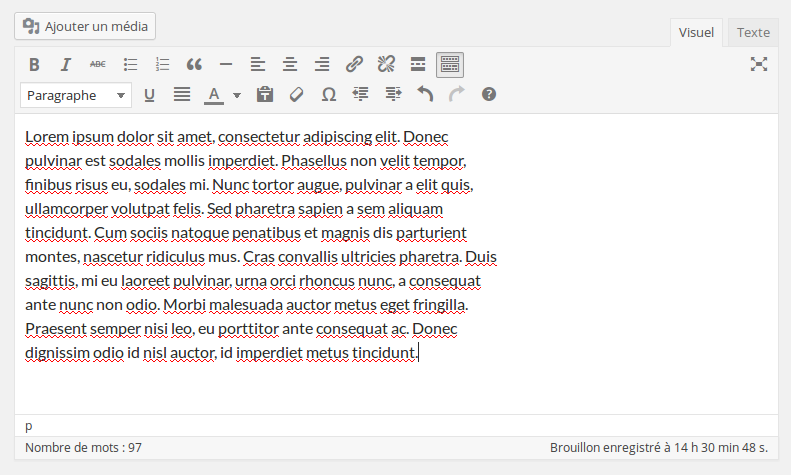
\includegraphics[scale=0.35]{img/0071.png}
\end{center}
\subsubsection{Les niveaux de titres}
Pour créer un titre ou un sous-titre, sélectionnez le texte puis choisissez le niveau de titre souhaité dans la liste des styles de formatage.
\begin{center}
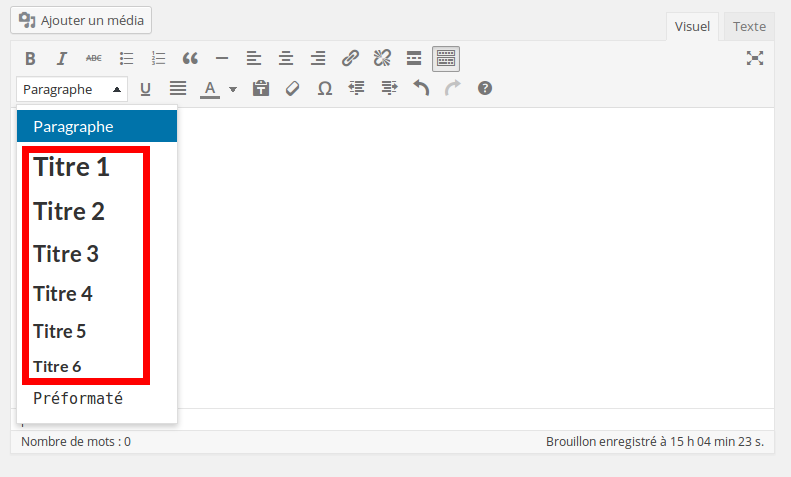
\includegraphics[scale=0.35]{img/0072.png}
\end{center}
\paragraph{}À noter que plus le chiffre est grand plus le titre est petit...
\subsubsection{Les listes à puces}
\paragraph{}Pour créer une liste à puces, sélectionnez les éléments de la liste puis cliquez sur le bouton « Liste à puces ».
\begin{center}
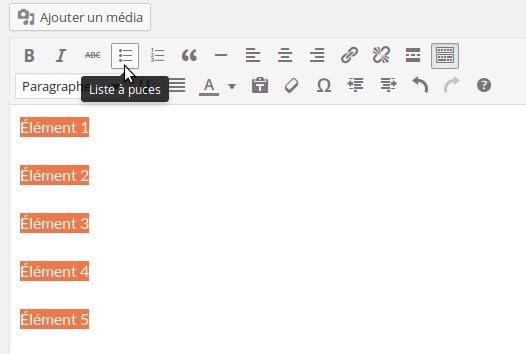
\includegraphics[scale=0.35]{img/0073.png}
\end{center}
\paragraph{}Vous obtiendrez une liste à puces.
\begin{center}
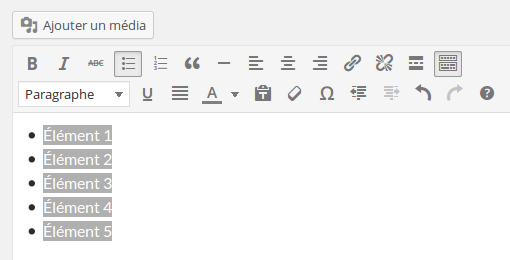
\includegraphics[scale=0.35]{img/0074.png}
\end{center}
\subsubsection{Les listes numérotées}
\paragraph{}Pour créer une liste numérotée, sélectionnez les éléments de la liste puis cliquez sur le bouton « Liste numérotée ».
\begin{center}
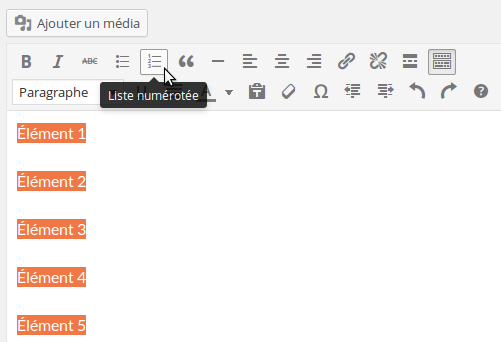
\includegraphics[scale=0.35]{img/0075.png}
\end{center}
\paragraph{}Vous obtiendrez une liste numérotée.
\begin{center}
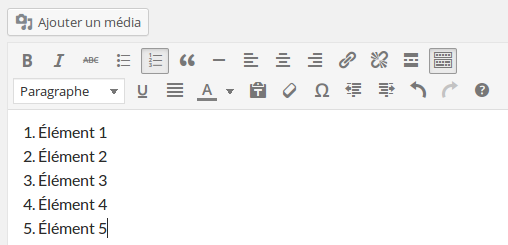
\includegraphics[scale=0.35]{img/0076.png}
\end{center}
\subsubsection{Les liens internes}
\paragraph{}Un lien interne est un lien qui renvoie vers une autre page de votre site. Pour créer un lien interne sélectionnez le texte à transformer en lien puis cliquez sur le bouton « Insérer/modifier un lien ».
\begin{center}
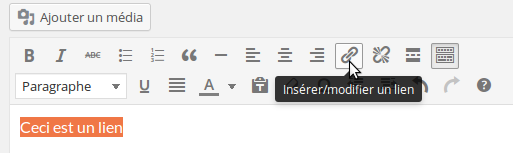
\includegraphics[scale=0.35]{img/0077.png}
\end{center}
\paragraph{}Dans la fenêtre qui apparaît, cliquez sur le bouton « Ou alors, faites un lien vers l'un des contenus de votre site » pour faire apparaître la liste des articles et pages de votre site.
\paragraph{}Sélectionnez l'article ou la page souhaitée puis cliquez sur le bouton « Ajouter un lien ».
\begin{center}
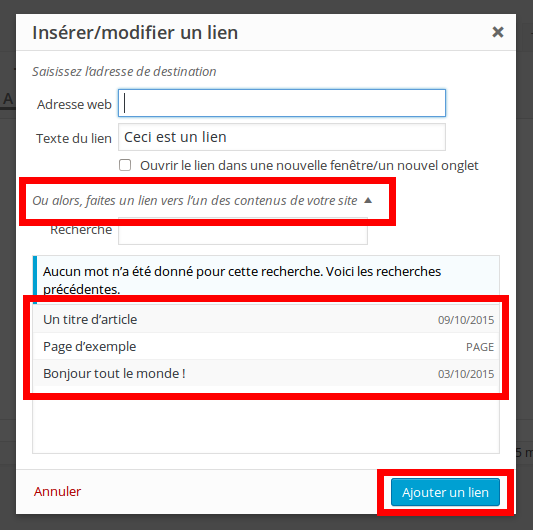
\includegraphics[scale=0.35]{img/0078.png}
\end{center}
\paragraph{}Votre lien est créé.
\begin{center}
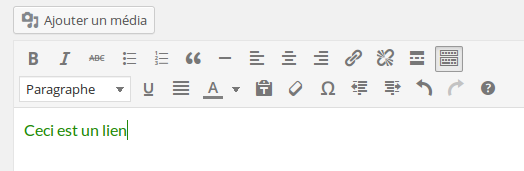
\includegraphics[scale=0.35]{img/0079.png}
\end{center}
\subsubsection{Les liens externes}
\paragraph{}Un lien externe est un lien qui renvoie vers un autre site Internet. Pour créer un lien externe sélectionnez le texte à transformer en lien puis cliquez sur le bouton « Insérer/modifier un lien ».
\begin{center}
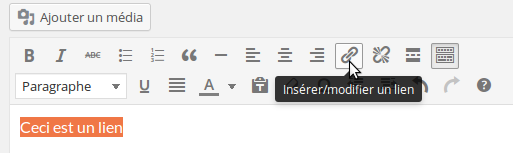
\includegraphics[scale=0.35]{img/0077.png}
\end{center}
\paragraph{}Dans la fenêtre qui apparaît, indiquez l'adresse complète (avec http://) du site, cochez la case « Ouvrir le lien dans une nouvelle fenêtre/un nouvel onglet » puis cliquez sur le bouton « Ajouter un lien ».
\begin{center}
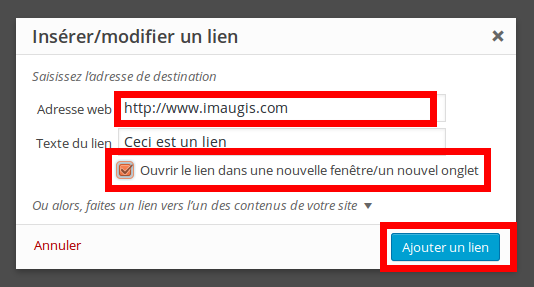
\includegraphics[scale=0.35]{img/0080.png}
\end{center}
\paragraph{}Votre lien est créé.
\begin{center}
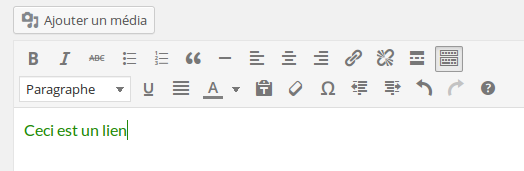
\includegraphics[scale=0.35]{img/0079.png}
\end{center}
\subsubsection{Les liens de téléchargement}
\paragraph{}Il est parfois utile de donner la possibilité à vos visiteurs de pouvoir télécharger certains documents (comme un bulletin d'adhésion par exemple). Pour créer un lien de téléchargement cliquez sur le bouton « Ajouter un média ».
\begin{center}
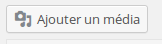
\includegraphics[scale=0.35]{img/0081.png}
\end{center}
\paragraph{}Vous accédez au gestionnaire de médias.
\paragraph{}Là, vous avez deux cas de figure possible :
\paragraph{}\textbf{Cas 1 : }Le fichier que vous souhaitez mettre en téléchargement se trouve déjà dans votre gestionnaire de médias et donc vous n'avez qu'à le sélectionner puis cliquer sur le bouton « Insérer dans l'article ».
\begin{center}
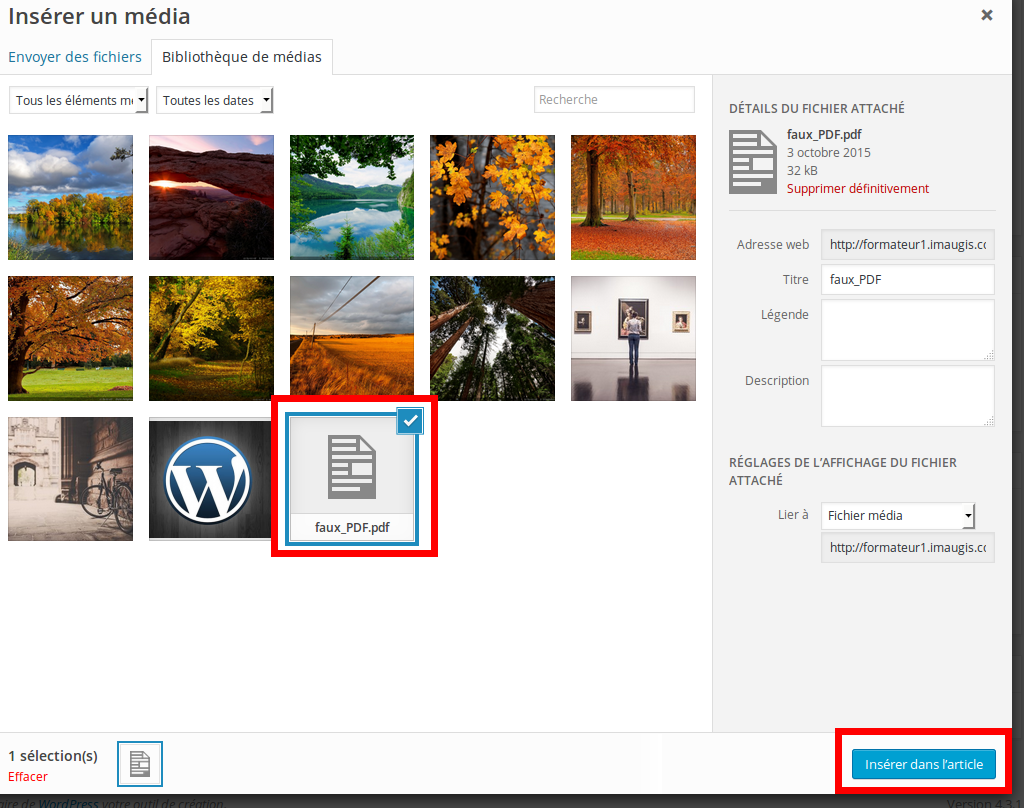
\includegraphics[scale=0.3]{img/0082.png}
\end{center}
\paragraph{}\textbf{Cas 2 : }Le fichier que vous souhaitez mettre en téléchargement ne se trouve pas dans votre gestionnaire de médias et donc vous allez devoir l'envoyer.
\paragraph{}Pour cela, cliquez sur l'onglet « Envoyer des fichiers ».
\begin{center}
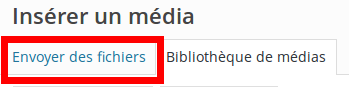
\includegraphics[scale=0.35]{img/0083.png}
\end{center}
\paragraph{}Cliquez ensuite sur le bouton « Choisir des fichiers » puis cherchez le fichier à mettre en téléchargement dans l'arborescence de votre ordinateur. Une fois le fichier trouvé, cliquez sur le bouton « Ouvrir » pour lancer l'envoie vers le gestionnaire de médias.
\begin{center}
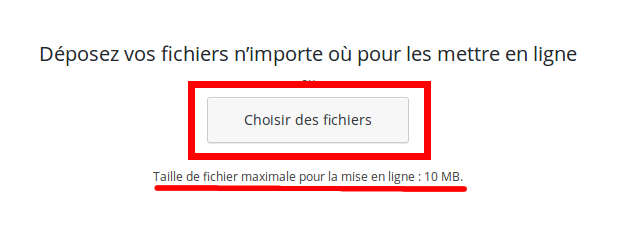
\includegraphics[scale=0.35]{img/0084.png}
\end{center}
\paragraph{}À noter que la taille maximale d'un fichier que vous pouvez envoyer est indiquée en dessous du bouton « Choisir des fichiers ».
\paragraph{}Une fois l'envoie terminé, le fichier envoyé est automatiquement sélectionné, vous n'avez plus qu'à cliquer sur le bouton « Insérer dans l'article ».
\begin{center}
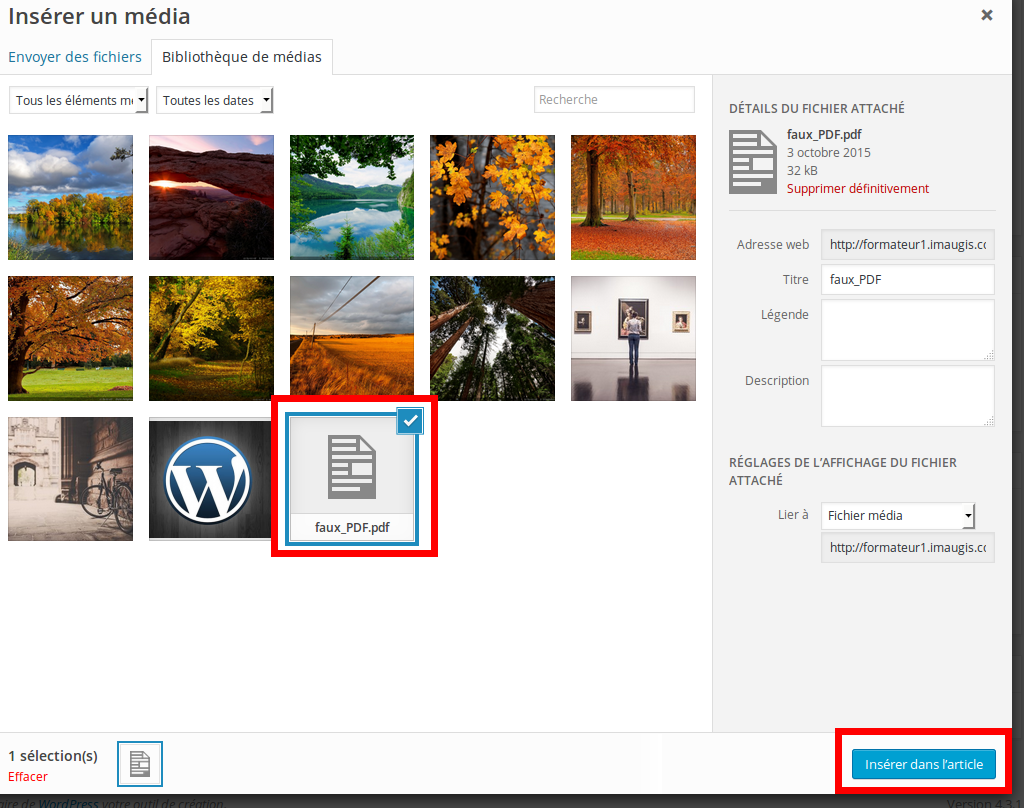
\includegraphics[scale=0.3]{img/0082.png}
\end{center}
\paragraph{}Le lien de téléchargement vers le fichier est créé cependant il prend, par défaut, le nom du fichier (sans l'extension). Il peut être judicieux de renommer le lien pour qu'il soit plus parlant. Pour cela, cliquez sur le lien. Vous devriez voir apparaître une infobulle en dessous de celui-ci. Cliquez sur le bouton « Modifier ».
\begin{center}
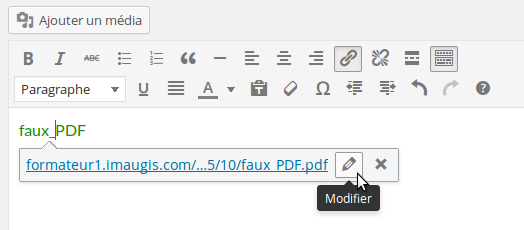
\includegraphics[scale=0.3]{img/0086.png}
\end{center}
\paragraph{}Dans la fenêtre qui apparaît, modifiez le champ « Texte du lien » puis cliquez sur le bouton « Mettre à jour » pour valider la modification.
\begin{center}
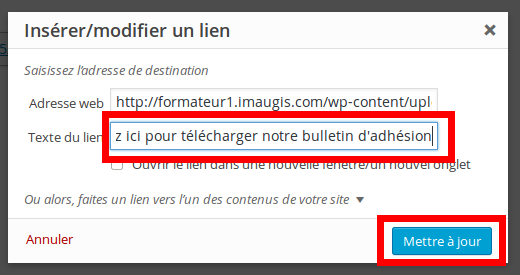
\includegraphics[scale=0.3]{img/0087.png}
\end{center}
\paragraph{}Et voilà, votre lien est désormais plus parlant ;)
\begin{center}
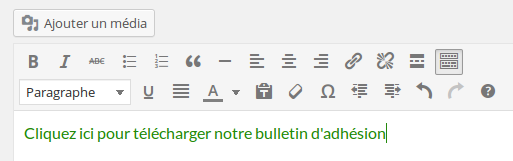
\includegraphics[scale=0.3]{img/0088.png}
\end{center}
\newpage

\section{Les médias}
\subsection{L'image à la une}
\paragraph{}L'image à la une est l'image qui va représenter un article ou une page. Elle s'affiche, en fonction du thème choisi, en premier plan (sur la page d'accueil et sur les pages de catégories d'articles. Il ne faut donc pas la négliger.
\subsubsection{Ajouter une image à la une}
\paragraph{}Pour ajouter une image à la une dans un article ou une page allez dans l'édition de cette dernière puis, dans la colonne de droite, en descendant, vous trouverez un bloc « Image à la une ».
\paragraph{}Cliquez sur le bouton « Mettre une image à la une ».
\begin{center}
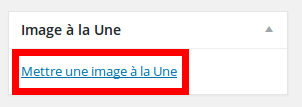
\includegraphics[scale=0.3]{img/0098.png}
\end{center}
\paragraph{}Dans le gestionnaire des médias, sélectionnez l'image souhaitée puis cliquez sur le bouton « Mettre une image à la une ». Si l'image souhaitée ne figure pas dans le gestionnaire des médias, cliquez sur l'onglet « Envoyer des fichiers » puis importez l'image depuis votre ordinateur.
\begin{center}
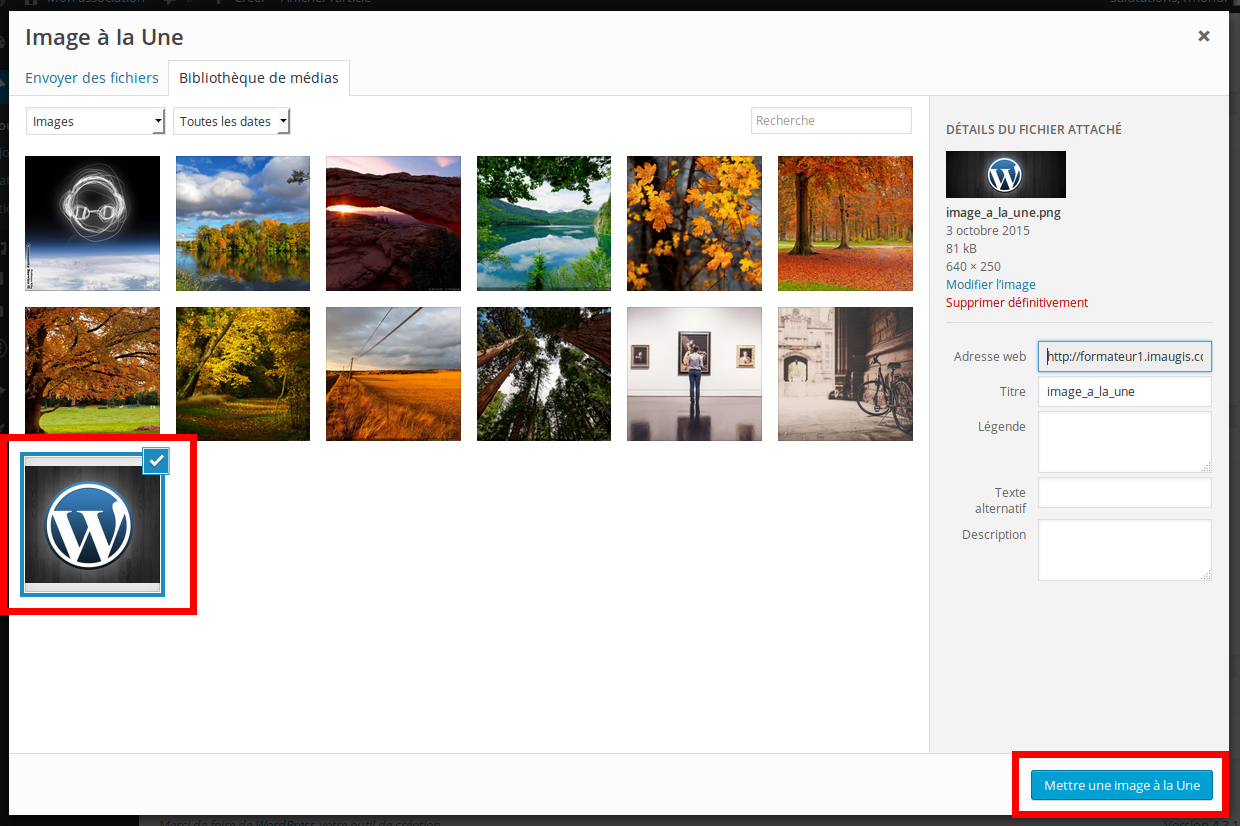
\includegraphics[scale=0.25]{img/0099.png}
\end{center}
\paragraph{}Si tout s'est bien passé vous devriez obtenir un aperçu de l'image à la une.
\begin{center}
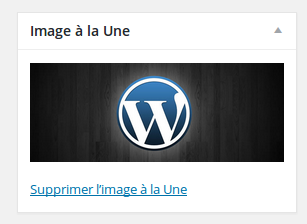
\includegraphics[scale=0.3]{img/0100.png}
\end{center}
\subsubsection{Supprimer une image à la une}
\paragraph{}Pour supprimer une image à la une, allez dans l'édition de l'article ou la page concernée puis, dans le bloc « Image à la une », cliquez sur le bouton « Supprimer l'image à la une ».
\begin{center}
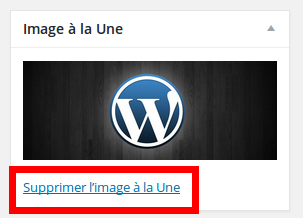
\includegraphics[scale=0.3]{img/0101.png}
\end{center}
\subsubsection{Recadrer une image à la une}
\paragraph{}Vous avez la possibilité de recadrer l'image à la une en fonction des différents formats utilisés sur votre site.
\paragraph{}Pour recadrer l'image à la une, cliquez sur « Recadrer l'image à la une ».
\begin{center}
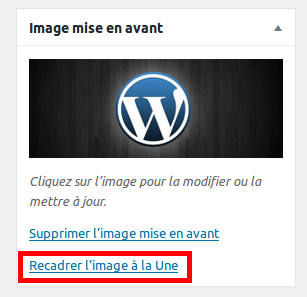
\includegraphics[scale=0.3]{img/0101b.png}
\end{center}
\paragraph{}Vous pouvez désormais recadrer votre image pour chaque format utilisé sur le site (slideshow, catégorie, article ou bien événement) à l'aide des différentes poignées apparaissant sur l'image. À noter que les proportions du format concerné seront conservées.
\begin{center}
\includegraphics[scale=0.3]{img/0101c.png}
\end{center}
\newpage
\subsection{Les images}
\paragraph{}En plus de l'image à la une, vous avez la possibilité d'agrémenter le corps de votre article ou de votre page d'images.
\subsubsection{Insérer une image dans le corps de l'article ou de la page}
\paragraph{}Pour insérer une image dans le corps d'un article ou d'une page, cliquez sur le bouton « Ajouter un média » situé au dessus de l'éditeur de texte.
\begin{center}
\includegraphics[scale=0.3]{img/0102.png}
\end{center}
\paragraph{}Dans le gestionnaire des médias, sélectionnez l'image souhaitée puis cliquez sur le bouton « Insérer dans l'article ». Si l'image souhaitée ne figure pas dans le gestionnaire des médias, cliquez sur l'onglet « Envoyer des fichiers » puis importez l'image depuis votre ordinateur.
\begin{center}
\includegraphics[scale=0.25]{img/0103.png}
\end{center}
\paragraph{}Si tout s'est bien passé, l'image sélectionnée est insérée dans le corps de l'article ou de la page.
\begin{center}
\includegraphics[scale=0.3]{img/0104.png}
\end{center}
\subsubsection{Redimensionner l'image}
\paragraph{}Cliquez sur l'image à redimensionner afin de faire apparaître les quatre poignées de redimensionnement.
\begin{center}
\includegraphics[scale=0.3]{img/0105.png}
\end{center}
\paragraph{}Cliquez sur l'une de ces poignées et tirez afin de redimensionner l'image à votre guise. À noter que les proportions seront toujours conservées.
\begin{center}
\includegraphics[scale=0.3]{img/0106.png}
\end{center}
\newpage
\subsubsection{L'alignement de l'image}
\paragraph{}Plusieurs options d'alignement s'offrent à vous :
\begin{itemize}
\item Centrer l'image
\item Aligner l'image à droite (avec contour de texte)
\item Aligner l'image à gauche (avec contour de texte)
\end{itemize}
\paragraph{Centrer l'image : }Pour centrer l'image, cliquez sur cette dernière afin de faire apparaître les option d'alignement.
\begin{center}
\includegraphics[scale=0.3]{img/0107.png}
\end{center}
\paragraph{}Cliquez sur le bouton « Centrer ».
\begin{center}
\includegraphics[scale=0.3]{img/0108.png}
\end{center}
\paragraph{}L'image est désormais centrée.
\begin{center}
\includegraphics[scale=0.3]{img/0109.png}
\end{center}
\paragraph{Aligner l'image à gauche : }Pour aligner l'image à gauche, cliquez sur cette dernière afin de faire apparaître les option d'alignement.
\begin{center}
\includegraphics[scale=0.3]{img/0107.png}
\end{center}
\paragraph{}À noter que pour faire passer le texte autour de l'image, ce dernier doit se trouver après l'image.
\paragraph{}Cliquez sur le bouton « Aligner à gauche ».
\begin{center}
\includegraphics[scale=0.3]{img/0110.png}
\end{center}
\paragraph{}L'image est désormais alignée à gauche et le texte passe autour.
\begin{center}
\includegraphics[scale=0.3]{img/0111.png}
\end{center}
\paragraph{Aligner l'image à droite : }Pour aligner l'image à droite, cliquez sur cette dernière afin de faire apparaître les option d'alignement.
\begin{center}
\includegraphics[scale=0.3]{img/0107.png}
\end{center}
\paragraph{}À noter que pour faire passer le texte autour de l'image, ce dernier doit se trouver après l'image.
\paragraph{}Cliquez sur le bouton « Aligner à droite ».
\begin{center}
\includegraphics[scale=0.3]{img/0112.png}
\end{center}
\paragraph{}L'image est désormais alignée à droite et le texte passe autour.
\begin{center}
\includegraphics[scale=0.3]{img/0113.png}
\end{center}
\newpage
\subsection{Insérer une galerie d'images}
\subsubsection{Créer une galerie d'images}
\paragraph{}Pour insérer une galerie d'image dans un article ou une page, cliquez sur le bouton « Ajouter un média » situé au dessus de l'éditeur de texte.
\begin{center}
\includegraphics[scale=0.3]{img/0102.png}
\end{center}
\paragraph{}Cliquez ensuite sur le bouton « Créer une galerie ».
\begin{center}
\includegraphics[scale=0.3]{img/0114.png}
\end{center}
\paragraph{}Sélectionnez les images souhaitées puis cliquez sur le bouton « Créer une nouvelle galerie ». Si les images souhaitées ne se trouvent pas dans le gestionnaire de médias, importez-les depuis votre ordinateur en cliquant sur l'onglet « Envoyer des fichiers ».
\begin{center}
\includegraphics[scale=0.25]{img/0115.png}
\end{center}
\paragraph{}Une fois la galerie créée, vous arrivez sur une page vous permettant de paramétrer la galerie avant de l'insérer sur l'article ou la page et notamment :
\begin{enumerate}
\item D'ajouter de nouvelles images
\item De modifier l'ordre des images en les faisant glisser / déposer là où vous le souhaitez
\item De supprimer des images de la galerie en cliquant sur la croix en haut à droite d'une miniature
\item De modifier le nombre de colonne (3 par défaut)
\end{enumerate}
\paragraph{}Une fois votre galerie paramétrée, cliquez sur le bouton « Insérer la galerie ».
\begin{center}
\includegraphics[scale=0.25]{img/0116.png}
\end{center}
\paragraph{}La galerie d'images est désormais insérée dans le corps de votre article ou de votre page.
\begin{center}
\includegraphics[scale=0.3]{img/0117.png}
\end{center}
\newpage
\subsubsection{Modifier une galerie d'images}
\paragraph{}Pour modifier une galerie d'images, cliquez une fois dessus afin de faire apparaître les options de modification et cliquez sur le bouton « Modifier ».
\begin{center}
\includegraphics[scale=0.3]{img/0118.png}
\end{center}
\paragraph{}Vous accédez à une page vous permettant de modifier la galerie et notamment :
\begin{enumerate}
\item D'ajouter de nouvelles images
\item De modifier l'ordre des images en les faisant glisser / déposer là où vous le souhaitez
\item De supprimer des images de la galerie en cliquant sur la croix en haut à droite d'une miniature
\item De modifier le nombre de colonne (3 par défaut)
\end{enumerate}
\paragraph{}Une fois votre galerie modifiée, cliquez sur le bouton « Mettre à jour la galerie ».
\begin{center}
\includegraphics[scale=0.25]{img/0116.png}
\end{center}
\newpage
\subsubsection{Supprimer une galerie d'images}
\paragraph{}Pour supprimer une galerie d'image, cliques une fois dessus pour faire apparaître les options de modification et cliquez sur le bouton « Supprimer ».
\begin{center}
\includegraphics[scale=0.3]{img/0119.png}
\end{center}
\newpage
\subsection{Insérer un fichier audio}
\paragraph{}Pour insérer un fichier audio dans un article ou une page, cliquez sur le bouton « Ajouter un média » situé au dessus de l'éditeur de texte.
\begin{center}
\includegraphics[scale=0.3]{img/0102.png}
\end{center}
\paragraph{}Dans le gestionnaire des médias, sélectionnez le fichier audio souhaité puis cliquez sur le bouton « Insérer dans l'article ». Si le fichier audio souhaité ne figure pas dans le gestionnaire des médias, cliquez sur l'onglet « Envoyer des fichiers » puis importez le depuis votre ordinateur.
\begin{center}
\includegraphics[scale=0.25]{img/0120.png}
\end{center}
\paragraph{}Si tout s'est bien passé, un lecteur audio est inséré dans le corps de l'article ou de la page.
\begin{center}
\includegraphics[scale=0.3]{img/0121.png}
\end{center}
\paragraph{}Et voilà, c'est aussi simple que ça !
\newpage
\subsection{Insérer une liste de lecture audio}
\paragraph{}Pour insérer une liste de lecture audio dans un article ou une page, cliquez sur le bouton « Ajouter un média » situé au dessus de l'éditeur de texte.
\begin{center}
\includegraphics[scale=0.3]{img/0102.png}
\end{center}
\paragraph{}Dans le gestionnaire des médias, cliquez sur le bouton « Créer une liste de lecture audio ».
\begin{center}
\includegraphics[scale=0.3]{img/0122.png}
\end{center}
\paragraph{}Sélectionnez les fichiers audio souhaités puis cliquez sur le bouton « Créer une nouvelle liste de lecture audio ». Si les fichiers audio souhaités ne figurent pas dans le gestionnaire des médias, cliquez sur l'onglet « Envoyer des fichiers » puis importez les depuis votre ordinateur.
\begin{center}
\includegraphics[scale=0.25]{img/0123.png}
\end{center}
\newpage
\paragraph{}Vous accédez à une page vous permettant de paramétrer la liste et notamment :
\begin{enumerate}
\item D'ajouter de nouveaux fichiers audio
\item De modifier l'ordre des fichiers audio en les faisant glisser / déposer là où vous le souhaitez
\item De supprimer des fichiers audio de la liste en cliquant sur la croix en haut à droite d'une miniature
\end{enumerate}
\paragraph{}Une fois votre liste paramétrée, cliquez sur le bouton « Insérer une liste de lecture audio ».
\begin{center}
\includegraphics[scale=0.25]{img/0124.png}
\end{center}
\paragraph{}Si tout s'est bien passé, un lecteur audio est inséré dans le corps de l'article ou de la page.
\begin{center}
\includegraphics[scale=0.3]{img/0125.png}
\end{center}
\newpage
\subsection{Insérer une vidéo}
\paragraph{}Pour insérer un fichier vidéo dans un article ou une page, cliquez sur le bouton « Ajouter un média » situé au dessus de l'éditeur de texte.
\begin{center}
\includegraphics[scale=0.3]{img/0102.png}
\end{center}
\paragraph{}Dans le gestionnaire des médias, sélectionnez le fichier vidéo souhaité puis cliquez sur le bouton « Insérer dans l'article ». Si le fichier vidéo souhaité ne figure pas dans le gestionnaire des médias, cliquez sur l'onglet « Envoyer des fichiers » puis importez le depuis votre ordinateur.
\begin{center}
\includegraphics[scale=0.25]{img/0126.png}
\end{center}
\paragraph{}Si tout s'est bien passé, un lecteur vidéo est inséré dans le corps de l'article ou de la page.
\begin{center}
\includegraphics[scale=0.3]{img/0127.png}
\end{center}
\newpage
\subsection{Insérer une liste de lecture vidéo}
\paragraph{}Pour insérer une liste de lecture vidéo dans un article ou une page, cliquez sur le bouton « Ajouter un média » situé au dessus de l'éditeur de texte.
\begin{center}
\includegraphics[scale=0.3]{img/0102.png}
\end{center}
\paragraph{}Dans le gestionnaire des médias, cliquez sur le bouton « Créer une liste de lecture vidéo ».
\begin{center}
\includegraphics[scale=0.3]{img/0128.png}
\end{center}
\paragraph{}Sélectionnez les fichiers vidéo souhaités puis cliquez sur le bouton « Créer une nouvelle liste de lecture vidéo ». Si les fichiers vidéo souhaités ne figurent pas dans le gestionnaire des médias, cliquez sur l'onglet « Envoyer des fichiers » puis importez les depuis votre ordinateur.
\begin{center}
\includegraphics[scale=0.25]{img/0129.png}
\end{center}
\newpage
\paragraph{}Vous accédez à une page vous permettant de paramétrer la liste et notamment :
\begin{enumerate}
\item D'ajouter de nouveaux fichiers vidéo
\item De modifier l'ordre des fichiers vidéo en les faisant glisser / déposer là où vous le souhaitez
\item De supprimer des fichiers vidéo de la liste en cliquant sur la croix en haut à droite d'une miniature
\end{enumerate}
\paragraph{}Une fois votre liste paramétrée, cliquez sur le bouton « Insérer une liste de lecture vidéo ».
\begin{center}
\includegraphics[scale=0.25]{img/0130.png}
\end{center}
\paragraph{}Si tout s'est bien passé, un lecteur vidéo est inséré dans le corps de l'article ou de la page.
\begin{center}
\includegraphics[scale=0.3]{img/0131.png}
\end{center}
\newpage
\subsection{Insérer une vidéo depuis une plate-forme externe}
\subsubsection{Insérer une vidéo depuis Youtube}
\paragraph{}Rendez-vous sur Youtube et copiez l'adresse complète de la page affichant la vidéo que vous souhaitez intégrer dans votre article ou votre page.
\begin{center}
\includegraphics[scale=0.3]{img/0132.png}
\end{center}
\paragraph{}Revenez sur l'édition de votre article ou de votre page et cliquez sur le bouton « Ajouter un média » situé au dessus de l'éditeur de texte.
\begin{center}
\includegraphics[scale=0.3]{img/0102.png}
\end{center}
\paragraph{}Cliquez ensuite sur le bouton « Insérer à partir d'une adresse web ».
\begin{center}
\includegraphics[scale=0.3]{img/0133.png}
\end{center}
\newpage
\paragraph{}Supprimez « http:// » dans le champs qui apparaît puis collez l'adresse que vous avez copié précédemment.
\begin{center}
\includegraphics[scale=0.3]{img/0134.png}
\end{center}
\paragraph{}Vous devriez voir apparaître un lecteur. Cliquez enfin sur le bouton « Insérer dans l'article ».
\begin{center}
\includegraphics[scale=0.25]{img/0135.png}
\end{center}
\paragraph{}Si tout s'est bien passé, un lecteur est inséré dans le corps de l'article ou de la page.
\begin{center}
\includegraphics[scale=0.3]{img/0136.png}
\end{center}
\newpage
\subsubsection{Insérer une vidéo depuis Dailymotion}
\paragraph{}Rendez-vous sur Dailymotion et copiez l'adresse complète de la page affichant la vidéo que vous souhaitez intégrer dans votre article ou votre page.
\begin{center}
\includegraphics[scale=0.3]{img/0137.png}
\end{center}
\paragraph{}Revenez sur l'édition de votre article ou de votre page et cliquez sur le bouton « Ajouter un média » situé au dessus de l'éditeur de texte.
\begin{center}
\includegraphics[scale=0.3]{img/0102.png}
\end{center}
\paragraph{}Cliquez ensuite sur le bouton « Insérer à partir d'une adresse web ».
\begin{center}
\includegraphics[scale=0.3]{img/0133.png}
\end{center}
\newpage
\paragraph{}Supprimez « http:// » dans le champs qui apparaît puis collez l'adresse que vous avez copié précédemment.
\begin{center}
\includegraphics[scale=0.3]{img/0134.png}
\end{center}
\paragraph{}Vous devriez voir apparaître un lecteur. Cliquez enfin sur le bouton « Insérer dans l'article ».
\begin{center}
\includegraphics[scale=0.25]{img/0138.png}
\end{center}
\paragraph{}Si tout s'est bien passé, un lecteur est inséré dans le corps de l'article ou de la page.
\begin{center}
\includegraphics[scale=0.3]{img/0139.png}
\end{center}
\newpage
\subsubsection{Insérer une vidéo depuis Vimeo}
\paragraph{}Rendez-vous sur Vimeo et copiez l'adresse complète de la page affichant la vidéo que vous souhaitez intégrer dans votre article ou votre page.
\begin{center}
\includegraphics[scale=0.3]{img/0140.png}
\end{center}
\paragraph{}Revenez sur l'édition de votre article ou de votre page et cliquez sur le bouton « Ajouter un média » situé au dessus de l'éditeur de texte.
\begin{center}
\includegraphics[scale=0.3]{img/0102.png}
\end{center}
\paragraph{}Cliquez ensuite sur le bouton « Insérer à partir d'une adresse web ».
\begin{center}
\includegraphics[scale=0.3]{img/0133.png}
\end{center}
\newpage
\paragraph{}Supprimez « http:// » dans le champs qui apparaît puis collez l'adresse que vous avez copié précédemment.
\begin{center}
\includegraphics[scale=0.3]{img/0134.png}
\end{center}
\paragraph{}Vous devriez voir apparaître un lecteur. Cliquez enfin sur le bouton « Insérer dans l'article ».
\begin{center}
\includegraphics[scale=0.25]{img/0141.png}
\end{center}
\paragraph{}Si tout s'est bien passé, un lecteur est inséré dans le corps de l'article ou de la page.
\begin{center}
\includegraphics[scale=0.3]{img/0142.png}
\end{center}
\newpage

\part{La gestion des formulaires}
\newpage

\section{Créer un formulaire}
\paragraph{}Rendez-vous dans Formidable > Formulaires.
\begin{center}
\includegraphics[scale=0.3]{img/0180.png}
\end{center}
\paragraph{}Cliquez sur le bouton « Modèles ».
\begin{center}
\includegraphics[scale=0.3]{img/0181.png}
\end{center}
\paragraph{}Passez votre souris sur le modèle « Contact Us » afin de faire apparaître des options supplémentaires puis cliquez sur le bouton « Créer un formulaire à partir du modèle ».
\begin{center}
\includegraphics[scale=0.3]{img/0182.png}
\end{center}
\paragraph{}Vous accédez au formulaire de création d'un... formulaire.
\paragraph{}Commencez par traduire le titre du formulaire puis la description de ce dernier.
\begin{center}
\includegraphics[scale=0.3]{img/0183.png}
\end{center}
\paragraph{}Traduisez les noms des champs qui sont, malheureusement en anglais par défaut.
\begin{center}
\includegraphics[scale=0.3]{img/0184.png}
\end{center}
\paragraph{}Vous avez la possibilité de supprimer des champs qui vous sembleraient inutiles en cliquant sur le bouton « Supprimer le champ » correspondant.
\begin{center}
\includegraphics[scale=0.3]{img/0185.png}
\end{center}
\paragraph{}Une fois ces réglages terminés, cliquez sur le bouton « Créer » pour valider la construction du formulaire.
\begin{center}
\includegraphics[scale=0.3]{img/0186.png}
\end{center}
\paragraph{}Vous accédez maintenant au paramétrage du formulaire.
\paragraph{Dans l'onglet « Général »} Traduisez le texte du bouton envoyer, le message de validation de soumission du formulaire puis cliquez sur le bouton « Mise à jour ».
\begin{center}
\includegraphics[scale=0.3]{img/0187.png}
\end{center}
\paragraph{Dans l'onglet « Actions du formulaire »} Cliquez sur « Email Notification » pour déplier les options puis modifiez si besoin le champ « à » qui comprend « [admin\_email] » ce qui correspond à l'adresse email de l'administrateur du site. Si cette adresse ne convient pas, supprimez « [admin\_email] » puis renseignez une adresse email à la place. Renseignez le sujet puis cliquez enfin sur le bouton « Mise à jour ».
\begin{center}
\includegraphics[scale=0.3]{img/0188.png}
\end{center}
\section{Insérer un formulaire sur une page}
\paragraph{}Rendez-vous dans Pages > Ajouter puis créez une page ayant comme titre, par exemple, « Nous contacter ».
\paragraph{}Cliquez sur le bouton « Formidable » situé au dessus de l'éditeur de texte.
\begin{center}
\includegraphics[scale=0.3]{img/0189.png}
\end{center}
\paragraph{}Sélectionnez le formulaire de contact dans la liste déroulante puis cliquez sur le bouton « Insérer dans l'article ».
\begin{center}
\includegraphics[scale=0.25]{img/0190.png}
\end{center}
\paragraph{}Le formulaire s'insère dans le corps de la page sous la forme d'un shortcode.
\begin{center}
\includegraphics[scale=0.3]{img/0191.png}
\end{center}
\paragraph{}Ajouter la page « Nous contacter » à votre menu principal puis allez la visiter. Vous devriez voir un joli formulaire de contact.
\begin{center}
\includegraphics[scale=0.3]{img/0192.png}
\end{center}
\newpage

\part{La gestion des événements}
\newpage

\section{Créer un nouvel événement}
\paragraph{}Pour créer un nouvel événement, rendez-vous dans Événements > Événements.
\begin{center}
\includegraphics[scale=0.3]{img/0196.png}
\end{center}
\paragraph{}Cliquez sur le bouton « Nouveau » pour ajouter un nouvel événement.
\begin{center}
\includegraphics[scale=0.3]{img/0197.png}
\end{center}
\newpage
\paragraph{}En plus du titre et du descriptif de l'événement, renseignez l'heure et la date, et le lieu de l'événement.
\begin{center}
\includegraphics[scale=0.3]{img/0198.png}
\end{center}
\paragraph{}À noter que chaque nouveau lieu sera sauvegardé et donc ne nécessitera pas de re-saisir ces informations lors d'un événement avec le même lieu.
\begin{center}
\includegraphics[scale=0.3]{img/0200.png}
\end{center}
\paragraph{}Une fois toutes ces informations dûment renseignées, cliquez sur le bouton « Publier » pour enregistrer le nouvel événement.
\paragraph{}Le nouvel événement est désormais affiché dans l'agenda.
\newpage
\section{Gérer les lieux}
\paragraph{}Comme je vous l'expliquais un peu plus haut, les lieux sont sauvegardés lorsqu'ils sont saisi pour la première fois.
\paragraph{}Il est possible de gérer et modifier ces lieux en vous rendant sur \textit{Événements > Lieux}.
\begin{center}
\includegraphics[scale=0.3]{img/0202.png}
\end{center}
\paragraph{}Passez ensuite votre souris sur le lieu à modifier ou supprimer afin de faire apparaître les options supplémentaires puis cliquez sur le bouton « Modifier » ou « Mettre à la corbeille » en fonction de votre besoin.
\begin{center}
\includegraphics[scale=0.3]{img/0203.png}
\end{center}
\newpage

\part{Les annuaires}
\newpage
\section{L'annuaire des associations}
\subsection{Lister les associations}
\paragraph{}Pour lister les associations, cliquez sur le bouton « Annuaire associations » dans le menu de gauche de votre site.
\begin{center}
\includegraphics[scale=0.3]{img/0298.png}
\end{center}
\paragraph{}Vous obtiendrez alors la liste complète des associations présentes sur votre site. Ces associations sont triées par défaut par date d'ajout (de la plus récente à la plus ancienne).
\begin{center}
\includegraphics[scale=0.3]{img/0299.png}
\end{center}
\subsection{Ajouter une nouvelle association}
\paragraph{}Pour ajouter une nouvelle association, cliquez sur... « Ajouter une nouvelle association ».
\begin{center}
\includegraphics[scale=0.3]{img/0300.png}
\end{center}
\paragraph{}Vous obtiendrez un formulaire pour ajouter une nouvelle association.
\begin{center}
\includegraphics[scale=0.3]{img/0301.png}
\end{center}
\paragraph{}Renseignez le nom de l'association, une description de cette dernière puis les paramètres supplémentaires de la structure.
\begin{center}
\includegraphics[scale=0.3]{img/0302.png}
\end{center}
\subsection{Éditer une association}
\paragraph{}Pour éditer une association, passez votre souris sur l’association en question afin de faire apparaître des options supplémentaires. Cliquez ensuite sur « Modifier ».
\begin{center}
\includegraphics[scale=0.3]{img/0303.png}
\end{center}
\paragraph{}Vous obtiendrez le formulaire pour éditer l'association.
\begin{center}
\includegraphics[scale=0.2]{img/0304.png}
\end{center}
\newpage
\subsection{Supprimer une association}
\paragraph{}Pour supprimer une association, passez votre souris sur l’association en question afin de faire apparaître des options supplémentaires. Cliquez ensuite sur « Corbeille ».
\begin{center}
\includegraphics[scale=0.3]{img/0305.png}
\end{center}
\paragraph{}Il est important de préciser que l’action « Mettre à la corbeille » n’est pas irréversible. En effet, vous pouvez rétablir une association, que vous auriez supprimé accidentellement par exemple, dans la corbeille.
\paragraph{}Si votre corbeille contient au moins un élément, vous verrez alors apparaître « Corbeille » suivi du nombre d’éléments qu’elle contient entre parenthèses au-dessus de la liste de vos associations.
\paragraph{}Cliquez sur le bouton « Corbeille » pour afficher la liste des associations qu’elle contient.
\begin{center}
\includegraphics[scale=0.35]{img/0069.png}
\end{center}
\paragraph{}Passez votre souris sur une association pour faire apparaître des options supplémentaires et cliquez sur « Rétablir » si vous souhaitez... rétablir une association supprimés accidentellement ou bien cliquez sur « Supprimer définitivement » si vous souhaitez... supprimer définitivement une association.
\paragraph{}À noter que vous pouvez \textbf{supprimer définitivement} le contenu de la corbeille en cliquant sur le bouton « Vider la corbeille ».
\begin{center}
\includegraphics[scale=0.35]{img/0070.png}
\end{center}
\newpage

\section{L'annuaire des artisans / commerçants}
\subsection{Lister les artisans / commerçants}
\paragraph{}Pour lister les artisans / commerçants, cliquez sur le bouton « Annuaire commerces » dans le menu de gauche de votre site.
\begin{center}
\includegraphics[scale=0.3]{img/0306.png}
\end{center}
\paragraph{}Vous obtiendrez alors la liste complète des artisans / commerçants présentes sur votre site. Ces artisans / commerçants sont triées par défaut par date d'ajout (de la plus récente à la plus ancienne).
\begin{center}
\includegraphics[scale=0.2]{img/0307.png}
\end{center}
\subsection{Ajouter un artisan / commerçant}
\paragraph{}Pour ajouter un nouvel artisan / commerçant, cliquez sur... « Ajouter un commerce/artisan ».
\begin{center}
\includegraphics[scale=0.3]{img/0308.png}
\end{center}
\paragraph{}Vous obtiendrez un formulaire pour ajouter un nouvel artisan / commerçant.
\begin{center}
\includegraphics[scale=0.2]{img/0309.png}
\end{center}
\paragraph{}Renseignez le nom de l'artisan / commerçant, une description de ce dernier puis les paramètres supplémentaires de la structure.
\begin{center}
\includegraphics[scale=0.3]{img/0310.png}
\end{center}
\subsection{Éditer un artisan / commerçant}
\paragraph{}Pour éditer un artisan / commerçant, passez votre souris sur l’artisan / commerçant en question afin de faire apparaître des options supplémentaires. Cliquez ensuite sur « Modifier ».
\begin{center}
\includegraphics[scale=0.3]{img/0311.png}
\end{center}
\paragraph{}Vous obtiendrez le formulaire pour éditer l'artisan / commerçant.
\begin{center}
\includegraphics[scale=0.3]{img/0312.png}
\end{center}
\newpage
\subsection{Supprimer un artisan / commerçant}
\paragraph{}Pour supprimer un artisan / commerçant, passez votre souris sur l’artisan / commerçant en question afin de faire apparaître des options supplémentaires. Cliquez ensuite sur « Corbeille ».
\begin{center}
\includegraphics[scale=0.3]{img/0313.png}
\end{center}
\paragraph{}Il est important de préciser que l’action « Mettre à la corbeille » n’est pas irréversible. En effet, vous pouvez rétablir un artisan / commerçant, que vous auriez supprimé accidentellement par exemple, dans la corbeille.
\paragraph{}Si votre corbeille contient au moins un élément, vous verrez alors apparaître « Corbeille » suivi du nombre d’éléments qu’elle contient entre parenthèses au-dessus de la liste de vos artisans / commerçants.
\paragraph{}Cliquez sur le bouton « Corbeille » pour afficher la liste des artisans / commerçants qu’elle contient.
\begin{center}
\includegraphics[scale=0.35]{img/0069.png}
\end{center}
\paragraph{}Passez votre souris sur un artisan / commerçant pour faire apparaître des options supplémentaires et cliquez sur « Rétablir » si vous souhaitez... rétablir un artisan / commerçant supprimés accidentellement ou bien cliquez sur « Supprimer définitivement » si vous souhaitez... supprimer définitivement un artisan / commerçant.
\paragraph{}À noter que vous pouvez \textbf{supprimer définitivement} le contenu de la corbeille en cliquant sur le bouton « Vider la corbeille ».
\begin{center}
\includegraphics[scale=0.35]{img/0070.png}
\end{center}
\newpage

\part{Les annonces immobilières}
\newpage

\subsection{Lister les annonces immobilières}
\paragraph{}Pour lister les annonces immobilières, cliquez sur le bouton « Annonces immobilières » dans le menu de gauche de votre site.
\begin{center}
\includegraphics[scale=0.3]{img/0314.png}
\end{center}
\paragraph{}Vous obtiendrez alors la liste complète des annonces immobilières présentes sur votre site. Ces offres immobilières sont triées par défaut par date d'ajout (de la plus récente à la plus ancienne).
\begin{center}
\includegraphics[scale=0.2]{img/0315.png}
\end{center}
\subsection{Ajouter une annonce immobilière}
\paragraph{}Pour ajouter une nouvelle annonce immobilière, cliquez sur... « Ajouter une annonce ».
\begin{center}
\includegraphics[scale=0.3]{img/0316.png}
\end{center}
\paragraph{}Vous obtiendrez un formulaire pour ajouter une nouvelle annonce immobilière.
\begin{center}
\includegraphics[scale=0.2]{img/0317.png}
\end{center}
\paragraph{}Renseignez le titre de l'annonce immobilière, une description de cette dernière puis les paramètres supplémentaires de l'annonce.
\begin{center}
\includegraphics[scale=0.3]{img/0318.png}
\end{center}
\subsection{Éditer une annonce immobilière}
\paragraph{}Pour éditer une annonce immobilière, passez votre souris sur l’annonce immobilière en question afin de faire apparaître des options supplémentaires. Cliquez ensuite sur « Modifier ».
\begin{center}
\includegraphics[scale=0.3]{img/0319.png}
\end{center}
\paragraph{}Vous obtiendrez le formulaire pour éditer l'annonce immobilière.
\begin{center}
\includegraphics[scale=0.2]{img/0320.png}
\end{center}
\newpage
\subsection{Supprimer une annonce immobilière}
\paragraph{}Pour supprimer une annonce immobilière, passez votre souris sur l’annonce immobilière en question afin de faire apparaître des options supplémentaires. Cliquez ensuite sur « Corbeille ».
\begin{center}
\includegraphics[scale=0.3]{img/0321.png}
\end{center}
\paragraph{}Il est important de préciser que l’action « Mettre à la corbeille » n’est pas irréversible. En effet, vous pouvez rétablir une annonce immobilière, que vous auriez supprimée accidentellement par exemple, dans la corbeille.
\paragraph{}Si votre corbeille contient au moins un élément, vous verrez alors apparaître « Corbeille » suivi du nombre d’éléments qu’elle contient entre parenthèses au-dessus de la liste de vos annonces immobilières.
\paragraph{}Cliquez sur le bouton « Corbeille » pour afficher la liste des annonces immobilières qu’elle contient.
\begin{center}
\includegraphics[scale=0.35]{img/0069.png}
\end{center}
\paragraph{}Passez votre souris sur une offre immobilière pour faire apparaître des options supplémentaires et cliquez sur « Rétablir » si vous souhaitez... rétablir une annonce immobilière supprimés accidentellement ou bien cliquez sur « Supprimer définitivement » si vous souhaitez... supprimer définitivement une annonce immobilière.
\paragraph{}À noter que vous pouvez \textbf{supprimer définitivement} le contenu de la corbeille en cliquant sur le bouton « Vider la corbeille ».
\begin{center}
\includegraphics[scale=0.35]{img/0070.png}
\end{center}
\newpage

\part{Les publications numériques}
\newpage

\section{Le magazine municipal}
\subsection{Ajouter un magazine municipal}
\paragraph{}Pour ajouter un nouveau magazine municipal cliquez sur le bouton « Magazine » situé dans le menu de gauche.
\begin{center}
\includegraphics[scale=0.3]{img/0322.png}
\end{center}
\paragraph{}Cliquez ensuite sur « Ajouter un magazine ».
\begin{center}
\includegraphics[scale=0.3]{img/0323.png}
\end{center}
\paragraph{}Vous obtiendrez un formulaire pour ajouter un nouveau magazine municipal.
\begin{center}
\includegraphics[scale=0.3]{img/0324.png}
\end{center}
\paragraph{}Renseignez le titre (\textit{Par exemple: Magazine numéro 42}), l'année de parution du magazine ainsi que la période du magazine.
\paragraph{}Cliquez enfin sur le bouton « Importer un magazine » afin d'aller rechercher le fichier PDF correspondant sur votre ordinateur.
\paragraph{Attention ! Les magazines municipaux sont triés par date de publication. Pensez à modifier cette date de publication en conséquence.}
\newpage

\section{Les comptes-rendus de conseils municipaux}
\subsection{Ajouter un compte-rendu de conseil municipal}
\paragraph{}Pour ajouter un nouveau compte-rendu de conseil municipal cliquez sur le bouton « Conseils Municipaux » situé dans le menu de gauche.
\begin{center}
\includegraphics[scale=0.3]{img/0325.png}
\end{center}
\paragraph{}Cliquez ensuite sur « Ajouter un compte-rendu ».
\begin{center}
\includegraphics[scale=0.3]{img/0326.png}
\end{center}
\paragraph{}Vous obtiendrez un formulaire pour ajouter un nouveau compte-rendu.
\begin{center}
\includegraphics[scale=0.3]{img/0327.png}
\end{center}
\paragraph{}Renseignez le titre (\textit{Par exemple: Séance du 17 octobre 2017}).
\paragraph{}Cliquez enfin sur le bouton « Importer un compte-rendu » afin d'aller rechercher le fichier PDF correspondant sur votre ordinateur.
\paragraph{Attention ! Les comptes-rendus de conseils municipaux sont triés par date de publication. Pensez à modifier cette date de publication en conséquence.}
\newpage

\part{La gestion des menus}
\newpage
\section{Créer un nouveau menu}
\subsection{Créer un nouveau menu}
\paragraph{}Pour créer un nouveau menu, rendez-vous dans Apparence > Menus.
\begin{center}
\includegraphics[scale=0.3]{img/0143.png}
\end{center}
\paragraph{}Cliquez sur le bouton « Créez un nouveau menu ».
\begin{center}
\includegraphics[scale=0.3]{img/0144.png}
\end{center}
\paragraph{}Renseignez le nom de votre menu (par exemple : menu principal) puis cliquez sur le bouton « Créer le menu ».
\begin{center}
\includegraphics[scale=0.3]{img/0145.png}
\end{center}
\paragraph{}Indiquez l'emplacement du thème dans lequel vous souhaitez placer votre menu (noms d'emplacement différents suivant les thèmes) puis cliquez sur le bouton « Enregistrer le menu ».
\begin{center}
\includegraphics[scale=0.3]{img/0146.png}
\end{center}
\paragraph{}Vous êtes désormais prêt à insérer des éléments dans votre menu.
\newpage
\subsection{Insérer une page dans le menu}
\paragraph{}Dans l'onglet « Pages », cliquez sur le bouton « Afficher tout » pour afficher toutes les pages de votre site.
\begin{center}
\includegraphics[scale=0.3]{img/0147.png}
\end{center}
\paragraph{}Sélectionnez la ou les pages à insérer dans le menu en cochant la ou les cases correspondantes puis cliquez sur le bouton « Ajouter au menu ».
\begin{center}
\includegraphics[scale=0.3]{img/0148.png}
\end{center}
\subsection{Insérer un lien personnalisé dans le menu}
\paragraph{}Dans l'onglet « Liens personnalisés », renseignez l'adresse complète (avec http://) du site vers lequel vous voulez créer un lien, renseignez ensuite le nom que prendra cet élément dans le menu puis cliquez enfin sur le bouton « Ajouter au menu ».
\begin{center}
\includegraphics[scale=0.3]{img/0149.png}
\end{center}
\subsection{Insérer une catégorie dans le menu}
\paragraph{}Dans l'onglet « Catégories », cliquez sur le bouton « Afficher tout » pour afficher toutes les catégories de votre site.
\begin{center}
\includegraphics[scale=0.3]{img/0150.png}
\end{center}
\paragraph{}Sélectionnez la ou les catégories à insérer dans le menu en cochant la ou les cases correspondantes puis cliquez sur le bouton « Ajouter au menu ».
\begin{center}
\includegraphics[scale=0.3]{img/0151.png}
\end{center}
\subsection{Créer un menu déroulant}
\paragraph{}Pour apprendre à créer un menu déroulant nous allons reprendre l'exemple de notre site de recettes de cuisine qui nous a été utile pour la gestion des catégories. Nous allons donc faire en sorte d'avoir un élément parent (les entrées) qui permettra d'afficher la liste des articles catégorisés « Les entrées » et donc obtenir la liste de toutes les recettes d'entrées (froides et chaudes). Puis nous allons y ajouter deux éléments enfants : Les entrées froides (qui permettra d'obtenir la liste des recettes d'entrées froides), et les entrées chaudes (qui permettra d'obtenir la liste des recettes des entrées chaudes).
\paragraph{}Commencez par ajouter l'élément parent (si ce n'est pas déjà fait).
\paragraph{}Dans l'onglet « Catégories », cliquez sur le bouton « Afficher tout » pour afficher toutes les catégories de votre site.
\begin{center}
\includegraphics[scale=0.3]{img/0150.png}
\end{center}
\paragraph{}Sélectionnez la catégorie « Les entrées » puis cliquez sur le bouton « Ajouter au menu ».
\begin{center}
\includegraphics[scale=0.3]{img/0151.png}
\end{center}
\paragraph{}Toujours dans l'onglet « Catégories », cliquez sur le bouton « Afficher tout » pour afficher toutes les catégories de votre site.
\begin{center}
\includegraphics[scale=0.3]{img/0150.png}
\end{center}
\paragraph{}Sélectionnez les catégories « Les entrées froides » et « Les entrées chaudes » puis cliquez sur le bouton « Ajouter au menu ».
\begin{center}
\includegraphics[scale=0.3]{img/0152.png}
\end{center}
\paragraph{}À ce stade, vous devez avoir les catégories « Les entrées froides » et « Les entrées chaudes » en dessous de la catégorie « Les entrées ».
\begin{center}
\includegraphics[scale=0.3]{img/0153.png}
\end{center}
\paragraph{}Pour créer un menu déroulant, les éléments enfants doivent se situer en dessous de l'élément parent (ce qui est déjà le cas) et être décalés d'un cran vers la droite (ce qui n'est pas encore le cas à ce stade).
\paragraph{}Pour décaler un élément, cliquez sur ce dernier sans relâcher puis décalez-le d'un cran vers la droite. Vous verrez des pointillés apparaître pour vous aider à visualiser le futur positionnement de votre élément. Quand ce dernier vous semble bon il suffit de relâcher le clic.
\begin{center}
\includegraphics[scale=0.3]{img/0154.png}
\end{center}
\paragraph{}Répétez l'opération pour chaque éléments enfants et voilà, votre menu déroulant est créé.
\begin{center}
\includegraphics[scale=0.3]{img/0155.png}
\end{center}
\newpage

\part{La gestion des utilisateurs}
\newpage
\section{Les rôles}
\paragraph{}Le système de Rôles a pour objectif de donner au propriétaire du blog la possibilité de contrôler et de déterminer ce que chaque utilisateur peut ou ne peut pas voir sur le blog. Un propriétaire de blog doit gérer et autoriser les accès à plusieurs fonctions comme la rédaction et l'édition de billets, la création de pages, la gestion des liens, la création des catégories, la modération des commentaires, la gestion des extensions, la gestion des thèmes, et la gestion des autres utilisateurs. Cet outil offre au propriétaire du blog, la possibilité d'attribuer un rôle à un utilisateur. 
\paragraph{}La notion de Rôles a été introduite à compter de la Version 2.0 de WordPress qui est livré 'de base' avec 5 rôles pré-définis : Administrateur, Éditeur, Auteur, Contributeur, and Abonné. Chaque rôle est pensé pour remplir plusieurs tâches appelées Permissions. Il y a trente Permissions dont la publication des billets, la modération des commentaires, et la gestion des utilisateurs. Les Permissions sont pré-déterminées pour chaque Rôle.
\paragraph{}Voici un aperçu des rôles et de leurs permissions dans votre site :
\begin{center}
\includegraphics[scale=0.5]{img/0156.png}
\end{center}
\newpage
\section{Ajouter, modifier ou supprimer un utilisateur}
\subsection{Ajouter un nouvel utilisateur}
\paragraph{}Pour ajouter un nouvel utilisateur rendez-vous dans Utilisateurs > Ajouter.
\begin{center}
\includegraphics[scale=0.3]{img/0157.png}
\end{center}
\paragraph{}Vous accédez à un formulaire vous demandant plusieurs renseignements :
\begin{itemize}
\item Identifiant (obligatoire) : C'est l'identifiant qui servira pour se connecter
\item E-mail (obligatoire) : L'adresse email du nouvel utilisateur
\item Prénom (optionnel) : Le prénom du nouvel utilisateur
\item Nom (optionnel) : Le nom du nouvel utilisateur
\item Site web (optionnel) : Si le nouvel utilisateur possède un site web, vous pouvez en indiquer l'adresse complète (avec http://) ici
\item Mot de passe (automatique) : Votre site va générer automatiquement un mot de passe pour le nouvel utilisateur. Ce dernier aura la possibilité de le modifier via un lien de réinitialisation de mot de passe qui lui sera envoyé dès que vous aurez validez l'ajout.
\item Rôle (obligatoire) : Sélectionnez le rôle qu'aura le nouvel utilisateur (Abonné par défaut)
\end{itemize}
\paragraph{}Une fois tous les champs correctement renseignés, cliquez sur le bouton « Ajouter un utilisateur ».
\begin{center}
\includegraphics[scale=0.3]{img/0158.png}
\end{center}
\paragraph{}Le nouvel utilisateur recevra un courriel l'informant de la création de son compte et lui permettant de réinitialiser son mot de passe.
\subsection{Modifier un utilisateur}
\paragraph{}Pour modifier un utilisateur rendez-vous dans Utilisateurs > Tous les utilisateurs pour accéder à la liste des utilisateurs.
\begin{center}
\includegraphics[scale=0.3]{img/0159.png}
\end{center}
\paragraph{}Passez votre souris au dessus de l'utilisateur à modifier pour faire apparaître des options supplémentaires puis cliquez sur le bouton « Modifier ».
\begin{center}
\includegraphics[scale=0.3]{img/0160.png}
\end{center}
\subsection{Supprimer un utilisateur}
\paragraph{}Pour supprimer un utilisateur rendez-vous dans Utilisateurs > Tous les utilisateurs pour accéder à la liste des utilisateurs.
\begin{center}
\includegraphics[scale=0.3]{img/0159.png}
\end{center}
\paragraph{}Passez votre souris au dessus de l'utilisateur à supprimer pour faire apparaître des options supplémentaires puis cliquez sur le bouton « Supprimer ».
\begin{center}
\includegraphics[scale=0.3]{img/0161.png}
\end{center}
\paragraph{}Votre site vous demande ce qu'il doit faire des éventuels publications de cet utilisateur. Deux choix s'offrent à vous :
\begin{itemize}
\item Supprimer tout le contenu de cet utilisateur
\item Attribuer tout le contenu de cet utilisateur à un autre utilisateur
\end{itemize}
\paragraph{}Je vous laisse le choix ;)
\paragraph{}Une fois votre choix effectué, cliquez sur le bouton « Confirmer la suppression » pour supprimer \textbf{définitivement} l'utilisateur.
\begin{center}
\includegraphics[scale=0.3]{img/0162.png}
\end{center}
\newpage

\end{document}
